\documentclass[a4paper, 11pt]{article}
\usepackage{comment} % enables the use of multi-line comments (\ifx \fi)  
\usepackage{fullpage} % changes the margin
\usepackage{mathtools} %allows us to write complex equations
\usepackage{graphicx} %allows us to add pictures
\usepackage{amsmath} %allows us to add Greek letters and equations
\usepackage{amssymb}
\usepackage{float} %formatting pictures
\usepackage{afterpage}
\usepackage{tikz}
\usetikzlibrary{automata, positioning, arrows}
\tikzset{->,>=stealth',node distance=3cm}

\begin{document}
\noindent
\large\textbf{Homework 2} \hfill \\
\large{Mike Gao} \\
\normalsize 260915701 \\
Prof. Prakash Panangaden \hfill 


\section*{Question 1}
Prove $F$ is not regular:
\begin{align*}
  F'  & =\overline{F} \cap ab^*c^* = \{ab^jc^k\mid j,k \geq 0 \text{ and } j \neq k \} \\
  F'' & =\overline{F'} \cap ab^*c^* = \{ab^rc^r\mid r \geq 0\}
\end{align*}

Since $\{a^nb^n|n\geq 0\}$ is not regular by pumping lemma, $F''$ is not regular, therefore, F is not regular.

Show that it satisfy the pumping lemma:
We choose $p=2$, So $\forall w\in L$ such that $|w| \geq p$, $w=xyz$ where $|y|\geq 1$ and $|xy| \leq p$, four cases:
\begin{enumerate}
\item $i = 0$, so $w=b^jc^k$. Then $y=b$ or $c$ is the first letter of the word, and $xy^nz=b^nb^{j-1}c^k \in L$ or $xy^nz=c^nc^{k-1} \in L$.
\item $i = 1$, so $j=k$, $w=ab^jc^j$. Set $y=a$ and $x=\epsilon$.  $w = a^nb^jc^j\in L$.
\item $i = 2$, so $w=a^2b^jc^k$. Set $y=aa$ and $x=\epsilon$.  $w=(aa)^nb^jc^k\in L$.
\item $i > 2$, so $w=a^ib^jc^k$. Set $y=a$ and $x=\epsilon$.  $w=a^{n}a^{i-1}b^jc^k\in L$.
\end{enumerate}

It satisfy the pumping lemma, but is in no way contradicting, since the pumping lemma states that all regular language can be pumped, not the other way around.

\section*{Question 2}
\subsection*{2.1}
False. Suppose $A = nil$ and B is any non regular language, clearly, $A\subseteq B$ but B not regular.
\subsection*{2.2}
False. Let $A= \{a^*\} \subseteq \Sigma^*$ be a regular language, $B=\{a^{2n}|n\geq0\}\subseteq{\Sigma^*}$ be a non regular language. AB and A are regular, but B clearly not.

\subsection*{2.3}
False. Counterexample: Assume $\Sigma=\{x,y\}$ The sets $S_1= \{xy\},S_2=\{xxyy\},S_3=\{xxxyyy\}$ etc are regular. While $\bigcup_{i=1}^{\inf}S_i=\{x^ny^n|n\geq 0\}$ But it is clearly not regular. So this is false.

\subsection*{2.4}
 False. Let A be some non regular language on a finite alphabet $\Sigma$ , thus $A \subseteq \Sigma^*$ and $\Sigma^*$ is regular.
 
\section*{Question 3}
\subsection*{3.1}
Let DFA $D=(S,s_0,F,\delta)$ be a DFA that recognizes L, now we construct a NFA $(Q,q_0,F',\delta)$ that recognizes $CYC(L)$. The state space of the NFA to be $Q=S \times S \times S \times \{0,1\}$ The first S tracks v, the second and third S guess where u start at, \{0,1\} tracks whether we're reading u or v.

Start state: $Q_0=\{(s_0,s,s,0) | s \in S\}$

Accepting state: $F^{'}=\{(s,t,s,1) \mid t\in F \}$

If $b=0$ and $\delta(t,a) \notin F$ then $\Delta((s,t,t_c,b),a) = \{(s,t',t_c,b)\mid t'=\delta(t,a)\}$.

If $b=0$ and $\delta(t,a) \in F$ then

\qquad$\Delta((s,t,t_c,b),a) = \{(s,t',t_c,b)\mid t'=\delta(t,a)\} \cup \{(s',t',t_c,b')\mid b'=1,t'=\delta(t,a)\}$

If $b=1$ then $\Delta((s,t,t_c,b),a) = \{(s',t,t_c,b)\mid s'=\delta(s,a)\}$.

This works because the end of $v$ will reach the start of $u$. $u$ will end in an accepting
state. So that $vu\in L$.

\subsection*{3.2}
Let $L=a^nba^n$, the language is not regular. $CYC(L)=a^mba^n,m+n\equiv0$ mod 2 which is regular since the following DFA recognizes it.

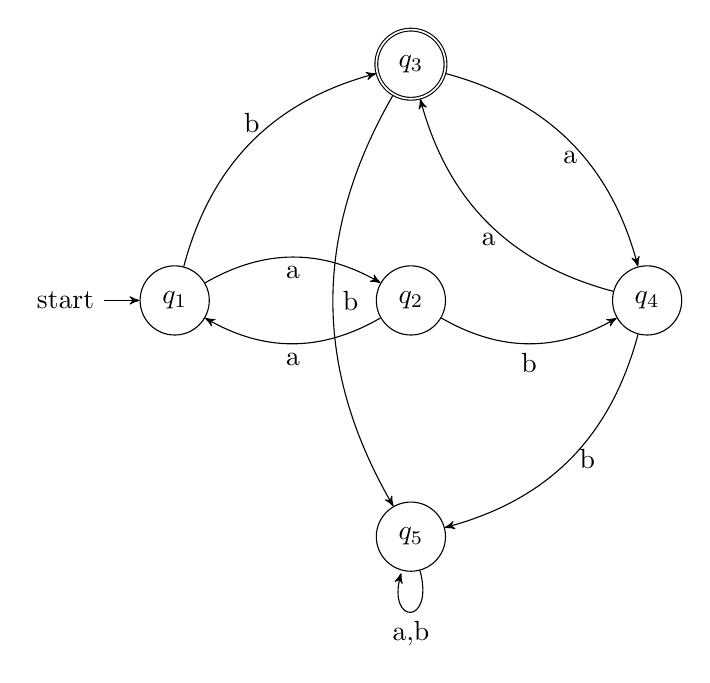
\begin{tikzpicture}
\node[state, initial] (q1) {$q_1$};
\node[state, right of=q1] (q2) {$q_2$};
\node[state, right of=q2] (q4) {$q_4$};
\node[state, accepting, above of=q2] (q3) {$q_3$};
\node[state, below of=q2] (q5) {$q_5$};
\draw 
(q1) edge[bend left, above] node{b} (q3)
(q1) edge[bend left, below] node{a} (q2)
(q2) edge[bend left, below] node{a} (q1)
(q3) edge[bend left, below] node{a} (q4)
(q2) edge[bend right, below] node{b} (q4)
(q3) edge[bend right, right] node{b} (q5)
(q4) edge[bend left, right] node{b} (q5)
(q5) edge[loop below] node{a,b} (q5)
(q4) edge[bend left, below] node{a} (q3);
\end{tikzpicture}



\section*{Question 4}
Counter example: Consider the following finite language $L=\{aa,ac,ba,bc,cb,db\}$, it is clear that $a \sim b$ $c \sim d$ However, it is false that $ac \sim bd$ since $ac \in L$ while $bd \notin L$. Hence $\equiv_L$ is not a congruence relation.

Show  $x \approx_L y \leftrightarrow \forall u,v \in \Sigma^*, uxv \in L  \leftrightarrow uyv \in L$

Let us assume that $x \approx_L y$ and $p \approx_L q$ Let us have arbitrary $u,v \in \Sigma^*$. Since we have $x\approx_L y$, $uxpv \in L \leftrightarrow uypv \in L$ Since we have $p \approx_L q$ we can get $uypv \in L \leftrightarrow uyqv \in L$ Hence we have $xp \approx_L yq$

\section*{Question 5}
\subsection*{5.1}
Not Equivalent.

\begin{align*}
     T=(\phi,\lnot,\psi) \rightarrow (\lnot\phi,\lnot \psi)\rightarrow (\lnot\phi,\lnot \psi)\rightarrow (\lnot\phi,\lnot \psi)\rightarrow\cdots
\end{align*}

$T\models (\square\lozenge\phi \implies \square\lozenge\psi)$ since the left side of the arrow is false, and false can imply anything.
  However, $T \not\models \square(\phi \implies \lozenge \psi)$.
  
\subsection*{5.2}
Not Equivalent

Let $T$ be a transition system where $\phi\land\lnot\psi$ for all odd step and $\lnot\phi\land\psi$ for all even step, $T\models\lozenge\phi\land\lozenge\psi$ however $T\not\models\lozenge(\phi\land\psi)$ since no step in $\phi$ and $\psi$ are both true.
\subsection*{5.3}
Equivalent
\begin{align*}
    \bigcirc\lozenge\phi & \equiv \bigcirc (\text{ true } U \phi) \\
                    & \equiv  (\bigcirc\text{ true }) U (\bigcirc\phi) \\
                    & \equiv \text{ true } U (\bigcirc\phi) \\
                    & \equiv \lozenge\bigcirc\phi
\end{align*}

\section*{Question 6}
\subsection*{6.1}
Formula : $\phi p = vX.p\land \bigcirc\bigcirc X$

\begin{align*}
    (\phi p)_0 & = \text{true} \\
    (\phi p)_1 & = p \\
    (\phi p)_2 & = p \land \bigcirc\bigcirc p \\
    (\phi p)_3 & = \text{true} \\
                     & \vdots  \\
    (\phi p)_n & = p \land \bigcirc \bigcirc p \land \bigcirc\bigcirc\bigcirc\bigcirc p \land \cdots \land \bigcirc^{n-1} p \\
\end{align*}
  
\subsection*{6.2}
Formula: $\star p = \mu X.p\land \bigcirc\bigcirc X$
\begin{align*}
    (\star p)_0 & = \text{false} \\
    (\star p)_1 & = p \land \bigcirc\bigcirc \text{false} \\
    & =\text{false}
\end{align*}

\subsection*{6.3}
Because it says immediately after a $p$ there is $\neg p$ and immediately after a $\neg p$ there is a $p$. Odd(P) doesn't necessarily have alternating p and $\neg p$ states.


\section*{Question 7}
Lets first analyze the effect of the binary operator $U$. Let $\phi=\psi_1 U \psi_2$ be a LTL formula. $\phi$ is true on $\sigma$ if there exists $j \geq 0$ such that $\delta[j...] \models \psi_2$ and for all $i < j$ $\delta[i...] \models \psi_1$ We can see that the truth value of $\phi$ depends on the existence of a state that satisfy $\psi_2$ after step $j \geq 0$ where all state before that satisfy $\psi_1$ no matter how many $U$ operators were added to $\phi$. The truth value stays the same for some $j \geq 0$
An example: let a and b be some states:
\begin{align*}
  (((a) \rightarrow (b) \rightarrow (a) \rightarrow (a) \rightarrow \cdots )\models \phi )
   & \equiv (((a) \rightarrow (a) \rightarrow (b) \rightarrow (a)\rightarrow (a) \rightarrow \cdots )\models \phi)                  \\
   & \equiv (((a) \rightarrow \cdots \rightarrow(a)\rightarrow (b) \rightarrow (a)\rightarrow (a) \rightarrow \cdots )\models \phi)
\end{align*}
Since $U$ has this property, other LTL operators such as $\square$ also has this property since they can be written as $U$, so, in a LTL formula $\phi$ with $U, \lozenge$ and $\square$ only,  $\phi$
has the same truth value on every $\sigma_i$ for $i\geq 0$.

Now lets discuss $\bigcirc$: Let $\phi=\bigcirc^i \psi$. We can see that the truth value of $\phi$ depends soly on $\sigma[i]$ since $\phi$ is true on $\sigma$ if $\sigma[i..]\models \psi$.

Consider a LTL formula $\phi$ with only $\bigcirc$ operators, since $\phi$ depends solely on $\sigma[i]$ and $\sigma[i]$ remains unchanged with variation of $j$, $\phi$ has the same truth value on every $\sigma_j$ for $j>i$.

Thus, given a proposition $p$ and any LTL formula $\phi$ containing $n$ next operators,
the fomula $\phi$ has the same truth value on every $\sigma_i$ with $i>n$.

Now, it is pretty clear that $odd(p)$ cannot be expressed in LTL.
Let's prove this by contradiction.
Assume it can be expressed in LTL $\phi$. Then $\phi$ must have a finite number of next operators. Assume $\phi$ has $n$ next operators. Then, by the statement we
proved earlier, $\sigma_i$ is true for all $i > n$ which is a contradiction since
one of $\sigma_{n+1}$ and $\sigma_{n+2}$ must be true, and the other one must be false.


\section*{Question 8}
\subsection*{8.1}
True. We want to show that both expression recognize the same language, such that:
$L_\omega ((E_1+E_2)\cdot F^\omega ) \equiv L_\omega (E_1 \cdot F^\omega + E_2 \cdot F^\omega)$

\begin{align*}
     L_\omega ((E_1+E_2)\cdot F^\omega ) &\equiv L_\omega (E_1+E_2) \cdot L_\omega(F^\omega) \\
     &\equiv (L_\omega(E_1) \cup L_\omega(E_2)) \cdot L_\omega(F^\omega) \\
     &\equiv \{xy| x\in{(L_\omega(E_1) \cup L_\omega(E_2))} \wedge y\in{L_\omega(F^\omega)}\} \\
     &\equiv \{xy| x\in{(L_\omega(E_1) \cup L_\omega(E_2))} \wedge y\in{L_\omega(F^\omega)}\} \\
     &\equiv \{xy| (x\in{L_\omega(E_1)}\wedge{y \in L_\omega(F^\omega)}) \vee (x\in{L_\omega(E_2)}\wedge{y \in L_\omega(F^\omega)}) \} \\
     &\equiv \{xy| x\in{L_\omega(E_1)}\wedge{y \in L_\omega(F^\omega)}\} \cup \{xy| x\in{L_\omega(E_2)}\wedge{y \in L_\omega(F^\omega)}\} \\
     &\equiv L_\omega(E_1\cdot F^\omega) \cup L_\omega(E_2\cdot F^\omega) \\
     &\equiv L_\omega(E_1\cdot F^\omega + E_2\cdot F^\omega)
\end{align*}

\subsection*{8.2}
False.
Let $E=\epsilon$, $F_1=x$, $F_2=y$. $xyxyxyxyxy... \in E\cdot (F_1+F_2)^\omega$ but $\notin E\cdot F_1^\omega + E\cdot F_2^\omega$

\subsection*{8.3}
False. Consider $E = x, F = y$ Then $(E^*F)^\omega \equiv (x^*y)^\omega$ while $E^*F^\omega \equiv x^*y^\omega$ $(x^*y)^\omega$ recognize word $xyxyxyxyxy....$ but $x^*y^\omega$ is incapable of recognizing the same word.

\section*{Question 9}
\subsection*{9.1}
$t_0 \models [a] \langle b \rangle true$ \\
$s_0 \not\models [a]  \langle b \rangle true$

The formula state that there exists a connected state over path a from which does not exist path b. $s_0$ satisfy this formula because the path from s0 to s3 doesn't have a b path, whereas $t_0$ does not satisfy it because a path leads to a state with b path.


\subsection*{9.2}
$t_0$ and $s_0$ agree on the following base case formulas:
true, $\langle a \rangle T$, $\langle b \rangle T$, $\langle a \rangle \langle\langle b \rangle T\rangle$ $\langle b \rangle \langle\langle a\rangle T\rangle$

By induction, they all should agree on any boolean combination of these formulas, for example, $t_0, s_0 \models (\langle a \rangle \text{true} ) \land (\langle a \rangle \langle b \rangle \text{true})$

\section*{Question 10}

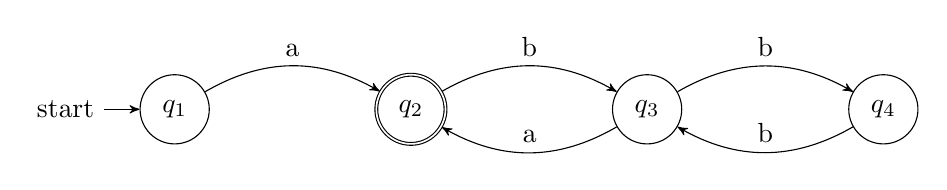
\begin{tikzpicture}
\node[state, initial] (q1) {$q_1$};
\node[state, accepting, right of=q1] (q2) {$q_2$};
\node[state, right of=q2] (q3) {$q_3$};
\node[state, right of=q3] (q4) {$q_4$};
\draw 
(q1) edge[bend left, above] node{a} (q2)
(q2) edge[bend left, above] node{b} (q3)
(q3) edge[bend left, above] node{a} (q2)
(q3) edge[bend left, above] node{b} (q4)
(q4) edge[bend left, above] node{b} (q3);
\end{tikzpicture}


\end{document}
